\documentclass[12pt]{article}

\usepackage{sbc-template}
\usepackage{graphicx,url}
\usepackage{multicol}
\usepackage{listings}
\usepackage{xcolor}
\usepackage[utf8]{inputenc}  

\definecolor{codegreen}{rgb}{0,0.6,0}
\definecolor{codegray}{rgb}{0.5,0.5,0.5}
\definecolor{codepurple}{rgb}{0.58,0,0.82}
\definecolor{backcolour}{rgb}{0.95,0.95,0.92}

\lstdefinestyle{mystyle}{
    backgroundcolor=\color{backcolour},   
    commentstyle=\color{codegreen},
    keywordstyle=\color{magenta},
    numberstyle=\tiny\color{codegray},
    stringstyle=\color{codepurple},
    basicstyle=\ttfamily\footnotesize,
    breakatwhitespace=false,         
    breaklines=true,                 
    captionpos=b,                    
    keepspaces=true,                 
    numbers=left,                    
    numbersep=5pt,                  
    showspaces=false,                
    showstringspaces=false,
    showtabs=false,                  
    tabsize=2
}

\lstset{style=mystyle}

\sloppy

\title{Unidade 01b - Noções de Complexidade}

\author{Luca Ribeiro Schettino Regne}

\begin{document} 

\maketitle

\section{Exercícios Resolvidos}

\subsection{Exercício Resolvido 1}
Calcule o número de subtrações que o código abaixo realiza:\\
\begin{lstlisting}[language=C]
  ...
  a--;
  a -= 3;
  a = 1 - 2;
\end{lstlisting}
3 subtrações.

\subsection{Exercício Resolvido 2}
Calcule o número de adições que o código abaixo realiza:
\begin{lstlisting}[language=C]
  ...
  if(a + 5 < b + 3)
    i++;
    ++b;
    a += 3;
  } else {
    j++;
  }
\end{lstlisting}
No melhor caso 3, no pior 5.

\subsection{Exercício Resolvido 3}
Calcule o número de adições que o código abaixo realiza:
\begin{lstlisting}[language=C]
  ...
  if(a + 5 < b + 3 || c + 1 < d + 3)
    i++;
    ++b;
    a += 3;
  } else {
    j++;
  }
\end{lstlisting}
No pior caso são executadas 7 somas, se e somente se a primeira sentença for falsa e a segunda verdadeira.
Enquanto no melhor caso são executadas 5 somas, quando as duas condições são falsas.

\subsection{Exercício Resolvido 4}
Calcule o número de subtrações que o código abaixo realiza:
\begin{lstlisting}[language=C]
  ...
  for(int i = 0; i < 4; i++){
    a--;
  }
\end{lstlisting}
São realizadas 4 subtrações.

\subsection{Exercício Resolvido 5}
Calcule o número de subtrações que o código abaixo realiza:
\begin{lstlisting}[language=C]
  ...
  for(int i = 0; i < n; i++){
    a--;
    b--;
  }
\end{lstlisting}
Serão realizadas 2n subtrações.

\subsection{Exercício Resolvido 6}
Calcule o número de subtrações que o código abaixo realiza:
\begin{lstlisting}[language=C]
  ...
  int i =0, b = 10;
  while(i < 3){
    i++;
    b--;
  }
\end{lstlisting}
Serão realizadas 3 subtrações.

\subsection{Exercício Resolvido 7}
Calcule o número de subtrações que o código abaixo realiza:
\begin{lstlisting}[language=C]
  ...
  for(int i = 3; i < n; i++){
    a--;
  }
\end{lstlisting}
Serão realizadas (n - 3) subtrações.

\subsection{Exercício Resolvido 8}
Calcule o número de subtrações que o código abaixo realiza:
\begin{lstlisting}[language=C]
  int a = 10;
  ...
  for(int i = 0; i < 3; i++){
    for(int j = 0; j < 2;j++){
      a--;
    }
  }
\end{lstlisting}
$3 * 2 = 6$\\
i = 0, j = 0\\
i = 0, j = 1\\
i = 1, j = 0\\
i = 1, j = 1\\
i = 2, j = 0\\
i = 2, j = 1\\
\\Serão realizadas 6 subtrações.

\subsection{Exercício Resolvido 9}
Calcule o número de multiplicações que o código abaixo realiza:
\begin{lstlisting}[language=C]
  ...
  for(int i = n; i < 0; i /= 2){
    a *= 2;
  }
\end{lstlisting}
Serão realizadas lg(n) + 1 multiplicações.

\subsection{Exercício Resolvido 10}
Faça um método que receba um número inteiro n e efetue o número de subtrações pedido em:\\
a)3n + 2n2\\
b)5n + 4n3\\
c)lg(n) + n\\
d)2n3 + 5\\
e)9n4 + 5n2 + n/2\\
f)lg(n) + 5 lg(n)
\begin{lstlisting}[language=C]
  i = 0;
  
  while (i < n){
    i++;a--;
    b--;
    c--;
  }
  
  for (i = 0;  i < n; i++){
    for (j = 0;  j < n; j++){
      a--;
      b--;
    }
  }
\end{lstlisting}

\subsection{Exercício Resolvido 11}
Encontre o menor valor em um array de inteiros
\begin{lstlisting}[language=C]
  int min = array[0];
  
  for (int i = 1; i < n; i++){
    if (min > array[i]){
      min = array[i];
    }
  }
\end{lstlisting}
1º) Qual é a operação relevante?\\
R: Comparação entre elementos do array.\\
2º) Quantas vezes ela será executada?\\
R: Se tivermos n elementos: T(n) = n - 1\\

\section{Exercícios}

\begin{multicols}{4}
  [
    \subsection{Exercício 1}
  ]
  a) $2^{0} = 1$ \\
  b) $2^{1} = 2$ \\
  c) $2^{2} = 4$ \\
  d) $2^{3} = 8$ \\
  e) $2^{4} = 16$ \\
  f) $2^{5} = 32$ \\
  g) $2^{6} = 64$ \\
  h) $2^{7} = 128$ \\
  i) $2^{8} = 256$ \\
  j) $2^{9} = 512$ \\
  k) $2^{10} = 1024$ \\
  l) $2^{11} = 2048$ \\
  \end{multicols}


\begin{multicols}{4}
  [
    \subsection{Exercício 2}
  ]
  a) $\log{2048} = 11$ \\
  b) $\log{1024} = 10$ \\
  c) $\log{512} = 9$ \\
  d) $\log{256} = 8$ \\
  e) $\log{128} = 7$ \\
  f) $\log{64} = 6$ \\
  j) $\log{32} = 5$ \\
  h) $\log{16} = 4$ \\
  i) $\log{8} = 3$ \\
  j) $\log{4} = 2$ \\
  k) $\log{2} = 1$ \\
  l) $\log{1} = 0$ \\
\end{multicols}

\begin{multicols}{4}
  [
    \subsection{Exercício 3}
  ]
  a) $\lceil 4,01 \rceil = 5$ \\
  b) $\lfloor 4,01 \rfloor = 4$ \\
  c) $\lceil 4,99 \rceil = 5$ \\
  d) $\lfloor 4,99 \rfloor = 4$ \\
  e) $\lceil \log{16} \rceil = 4$ \\
  f) $\lfloor \log{16} \rfloor = 4$ \\
  g) $\log{17} = 4.08$ \\
  h) $\lceil \log{17} \rceil = 4$ \\
  i) $\lfloor \log{17} \rfloor = 5$ \\
  j) $\log{15} = 3.90$ \\
  k) $\lceil \log{15} \rceil = 3$ \\
  l) $\lfloor \log{15} \rfloor = 4$ \\
  
\end{multicols}
  
\subsection{Exercício 4}
  a) $f(n) = n$
  \begin{center}
    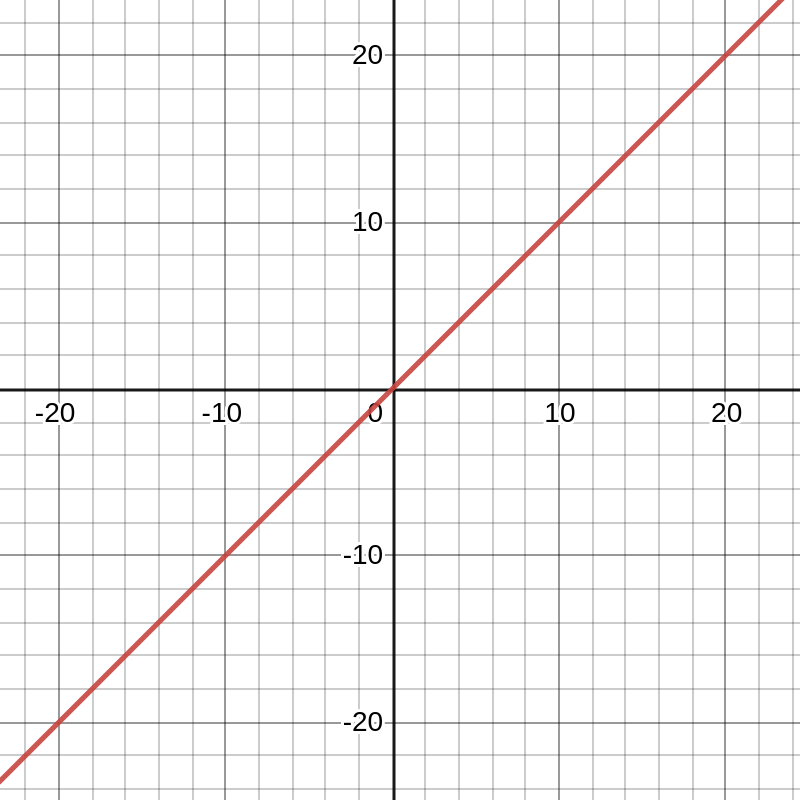
\includegraphics[width=0.7\textwidth]{graphics/a.png}
  \end{center}
  b) $f(n) = n^{2}$
  \begin{center}
    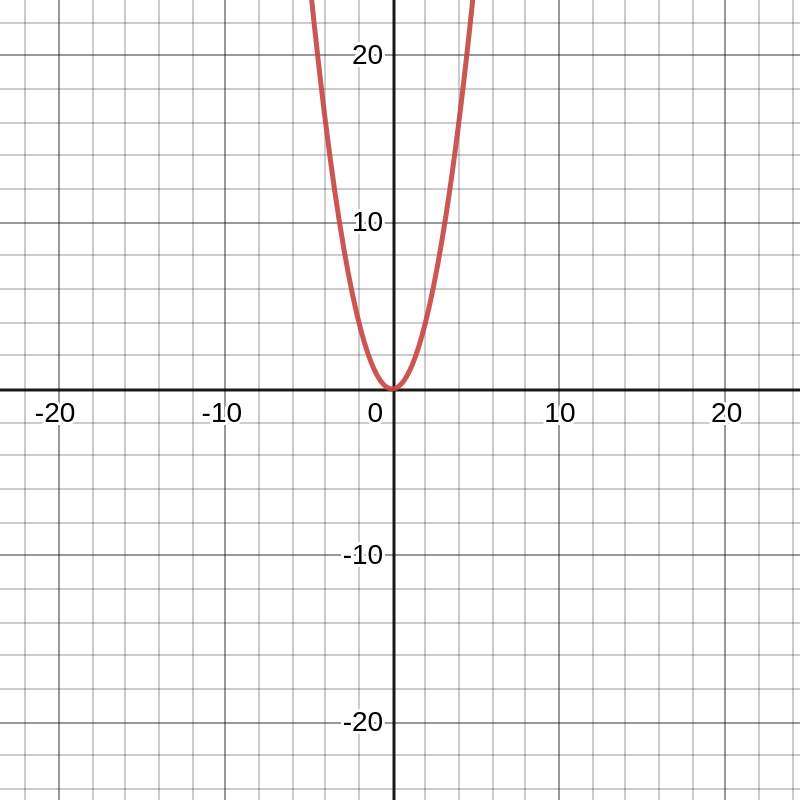
\includegraphics[width=0.7\textwidth]{graphics/b.png}\\
  \end{center}
  c) $f(n) = n^{3}$
  \begin{center}
    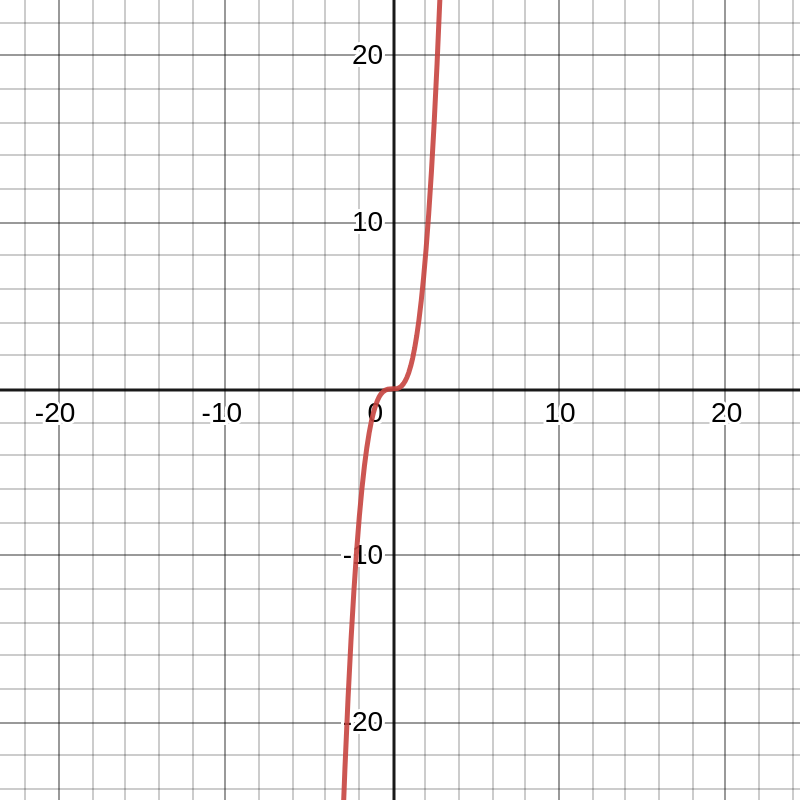
\includegraphics[width=0.7\textwidth]{graphics/c.png}\\
  \end{center}
  d) $f(n) = sqrt(n)$
  \begin{center}
    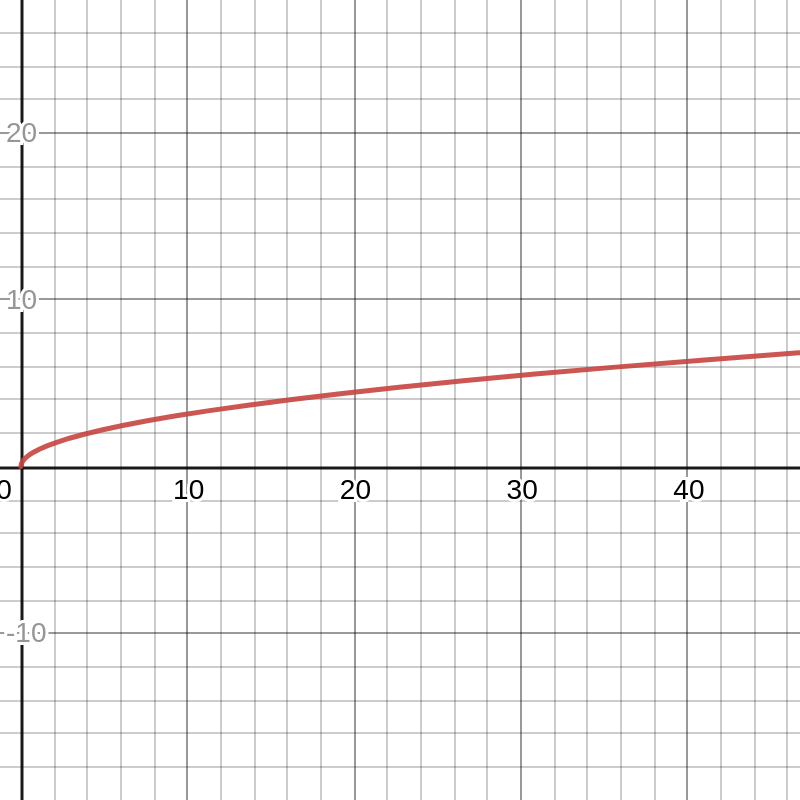
\includegraphics[width=0.7\textwidth]{graphics/d.png}\\
  \end{center}
  e) $f(n) = \lg{n} = \log_{2}{n}$
  \begin{center}
    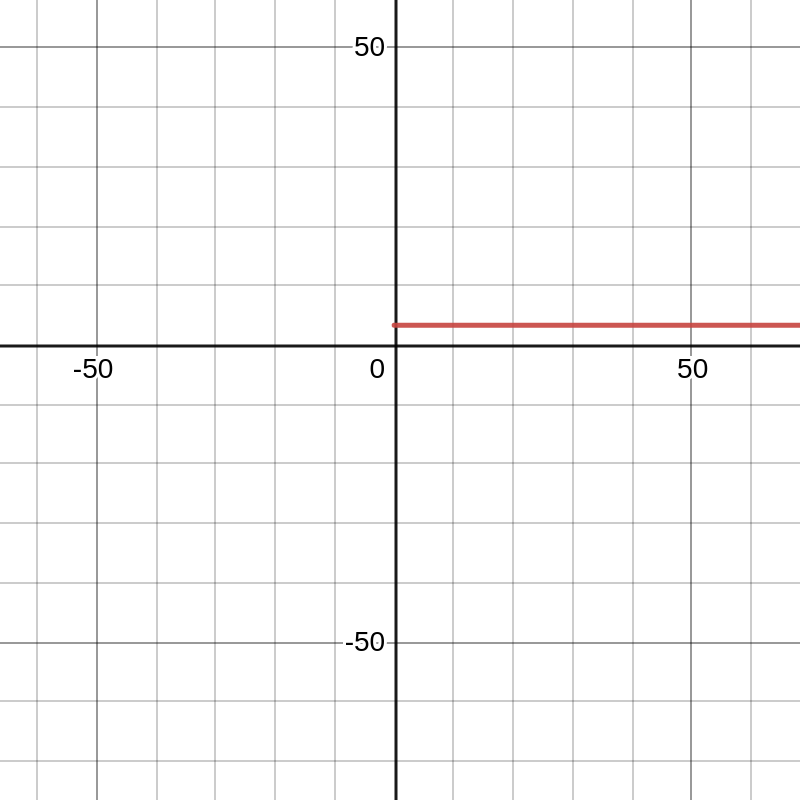
\includegraphics[width=0.7\textwidth]{graphics/e.png}\\
  \end{center}
  f) $f(n) = 3n^{2} + 5n - 3$
  \begin{center}
    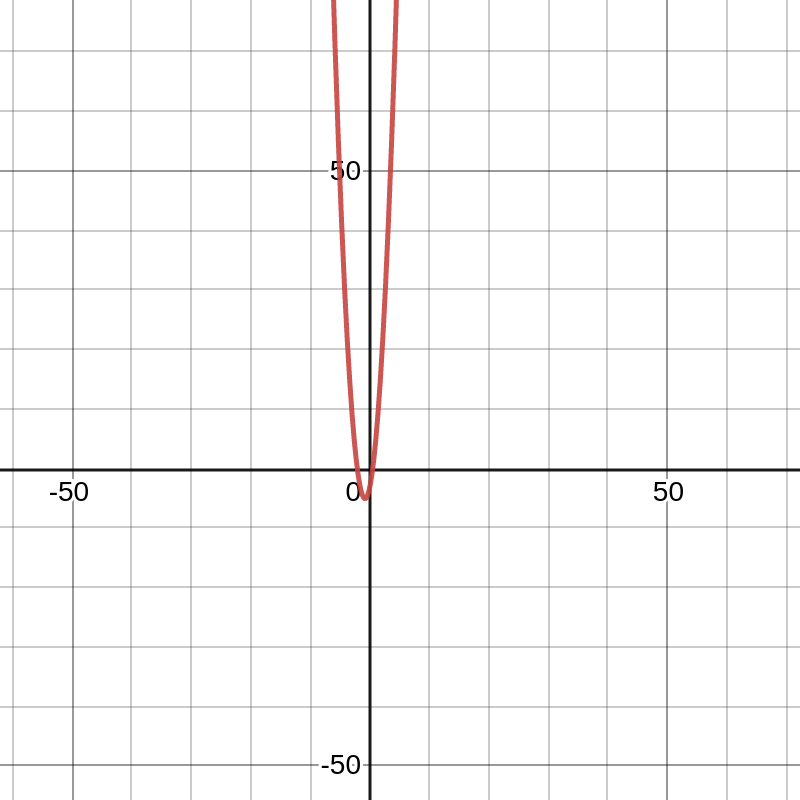
\includegraphics[width=0.7\textwidth]{graphics/f.png}\\
  \end{center}
  g) $f(n) = -3n^{2} + 5n - 3$
  \begin{center}
    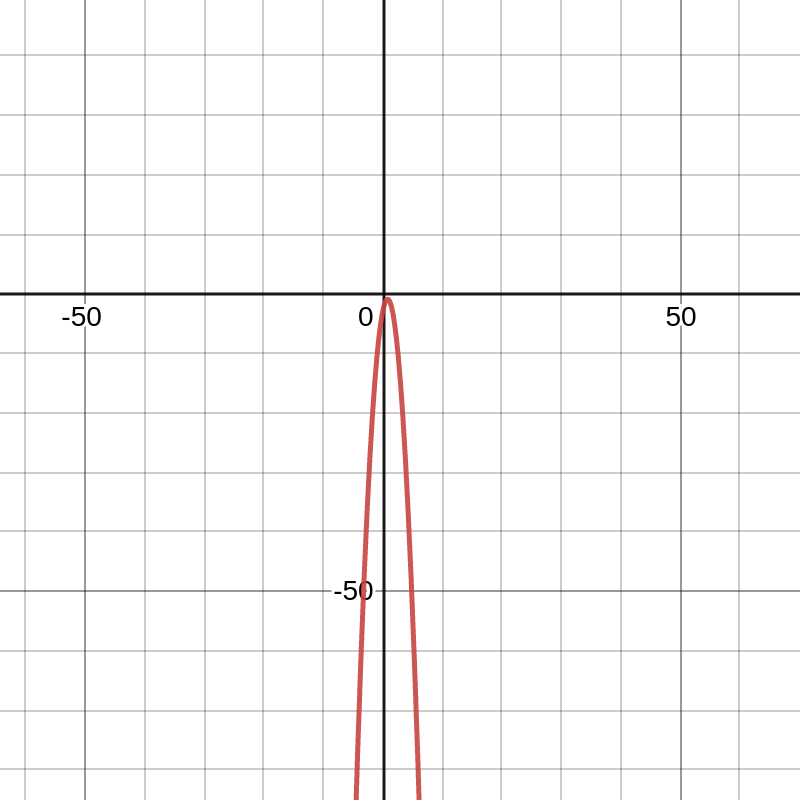
\includegraphics[width=0.7\textwidth]{graphics/g.png}\\
  \end{center}
  h) $f(n) = |-n^{2}|$
  \begin{center}
    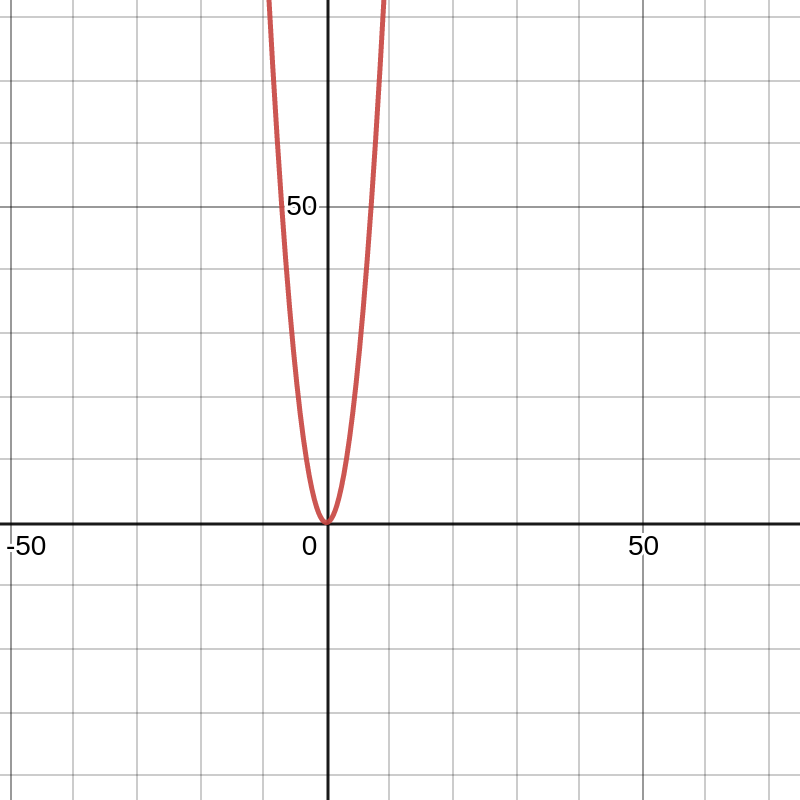
\includegraphics[width=0.7\textwidth]{graphics/h.png}\\
  \end{center}
  i) $f(n) = 5n^{4} + 2n^{2}$
  \begin{center}
    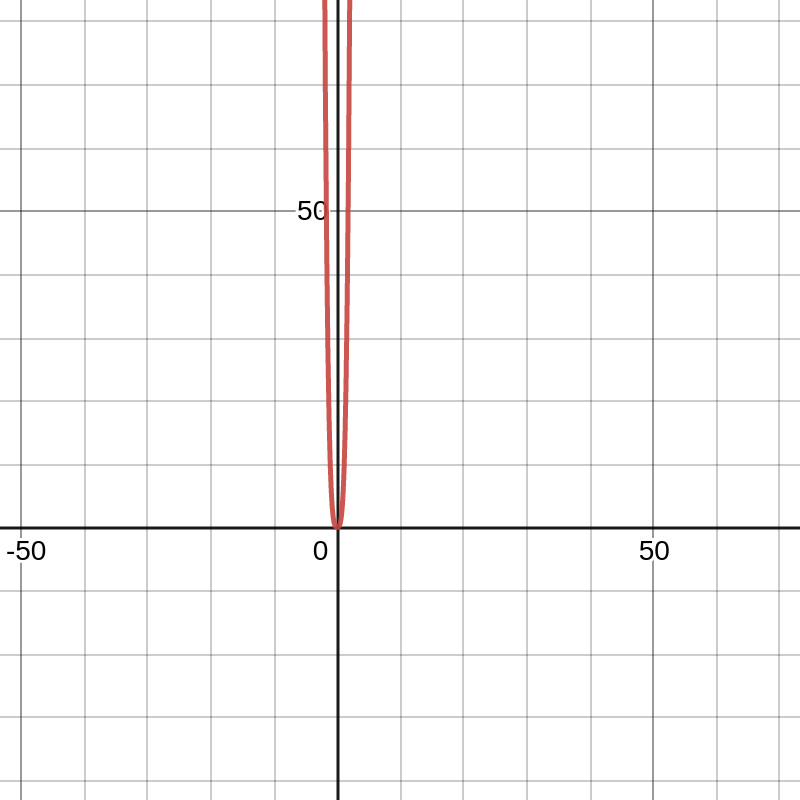
\includegraphics[width=0.7\textwidth]{graphics/i.png}\\
  \end{center}
  j) $f(n) = n * \lg{(n)}$
  \begin{center}
    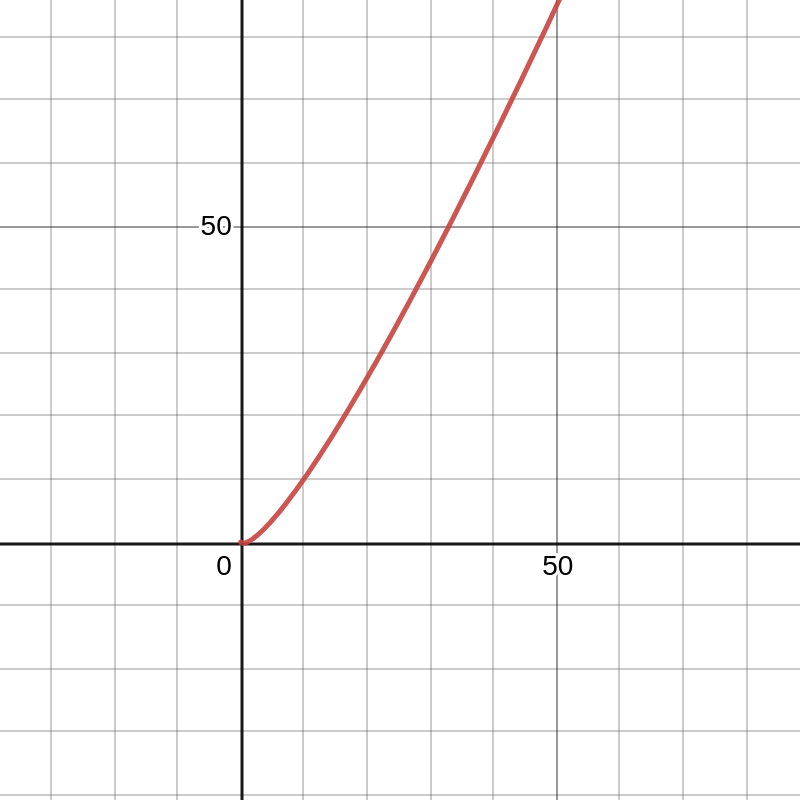
\includegraphics[width=0.7\textwidth]{graphics/j.png}\\
\end{center}


\subsection{Exercício 5}
Calcule o número de subtrações que o código abaixo realiza:
\begin{lstlisting}[language=C]
  ...
  int i = 10;
  while(i >= 7){
    i--;
  }
\end{lstlisting}
Serão realizadas 4 subtrações, quando i valer 10, 9, 8 e 7.

\subsection{Exercício 6}
Calcule o número de subtrações que o código abaixo realiza:
\begin{lstlisting}[language=C]
  ...
  for(int i = 5; i >- 2; i--){
    a--;
  }
\end{lstlisting}
($5-2 + 1) * 2 = (3+1) * 2 = 4 * 2 = 8$\\
Serão realizadas 8 subtrações. 

\subsection{Exercício 7}
Calcule o número de subtrações que o código abaixo realiza:
\begin{lstlisting}[language=C]
  ...
  for (int i = 0; i < 5; i++){
    if (i % 2 == 0){
      a--;
      b--;
    } else{
      c--;
    }
  }
\end{lstlisting}
0, 2, 4 -> 2 \\
1, 3 -> 1 \\
$3 * 2 * 2 * 1 = 6 + 1 = 7$ \\
Serão realizadas 7 subtrações.


\subsection{Exercício 8}
Calcule o número de subtrações que o código abaixo realiza:
\begin{lstlisting}[language=C]
  ...
  for (int i = 0; i < n; i++){
    for (int j = 0; j < n; j++){
      a--;
    }
  }
\end{lstlisting}
Serão realizadas $n^2$ subtrações.

\subsection{Exercício 9}
Calcule o número de subtrações que o código abaixo realiza:
\begin{lstlisting}[language=C]
  ...
  int i = 1, b = 10;
  while (i > 0){
    b--;
    i = i >> 1;
  }
  i = 0;
  while (i < 15){
    b--;
    i += 2;
  }
\end{lstlisting}
$1 + 15/2 = 1 + 7 = 8$\\
Serão realizadas 8 subtrações.

\subsection{Exercício 10}
Calcule o número de multiplicações que o código abaixo realiza:
\begin{lstlisting}[language=C]
  ...
  for (int i = 0; i < n; i++)
    for (int j = 0; j < n - 3; j++)
      a *= 2;
\end{lstlisting}
$n*(n - 3)$\\
Serão realizadas n*(n - 3) multiplicações.

\subsection{Exercício 11}
Calcule o número de multiplicações que o código abaixo realiza:
\begin{lstlisting}[language=C]
  ...
  for (int i = n - 7; i >= 1; i--)
    for (int j = 0; j < n; j++)
      a *= 2;

\end{lstlisting}
$((n - 7) - 1) * (n) = n * (n - 8)$\\
Serão realizadas n*(n-8) multiplicações.

\subsection{Exercício 12}
Calcule o número de multiplicações que o código abaixo realiza:
\begin{lstlisting}[language=C]
  ...
  for (int i = n; i > 0; i /= 2)
      a *= 2;

\end{lstlisting}
Serão realizadas $\log_{2}{n} + 1$ multiplicações.

\subsection{Exercício 13}
Calcule o número de multiplicações que o código abaixo realiza:
\begin{lstlisting}[language=C]
  ...
  for (int i = n+4; i > 0; i >>= 1)
    a *= 2;
\end{lstlisting}
Serão realizadas $\log_{2}{n+4}$ multiplicações.

\subsection{Exercício 14}
Calcule o número de multiplicações que o código abaixo realiza:
\begin{lstlisting}[language=C]
  ...
  for (int i = n - 7; i >= 1; i--)
    for (int j = n - 7; j >= 1; j--)
      a *= 2;

\end{lstlisting}
Serão realizadas $(n - 7)^2$ multiplicações.

\bibliographystyle{sbc}
\bibliography{sbc-template}

\subsection{Exercício 15}
Calcule o número de multiplicações que o código abaixo realiza:
\begin{lstlisting}[language=C]
  ...
  for (int i = n + 1; i > 0; i /= 2)
    a *= 2;
\end{lstlisting}
Serão realizadas $(\lg{n+1}2$ multiplicações.

\bibliographystyle{sbc}
\bibliography{sbc-template}

\subsection{Exercício 16}
Calcule o número de multiplicações que o código abaixo realiza:
\begin{lstlisting}[language=C]
  ...
  for (int i = n; i > 1; i /= 2)
    a *= 2
\end{lstlisting}
Serão realizadas $\lg{n}$ multiplicações.

\bibliographystyle{sbc}
\bibliography{sbc-template}

\subsection{Exercício 17}
Calcule o número de multiplicações que o código abaixo realiza:
\begin{lstlisting}[language=C]
  ...
  for (int i = 1; i < n; i *= 2)
    a *= 2;
\end{lstlisting}
Serão realizadas $(\sqrt{n}*2)$ multiplicações.

\subsection{Exercício 18}
Calcule o número de multiplicações que o código abaixo realiza:
\begin{lstlisting}[language=C]
  ...
  for (int i = 1; i <= n; i*= 2)
    a *= 2;
\end{lstlisting}
Serão realizadas $((\sqrt{n}+1)*2)$ multiplicações.

\bibliographystyle{sbc}
\bibliography{sbc-template}

\end{document}